\section{Images of Test Subject During Experiments}
\label{sec:Images of Test Subject During Experiments}

\begin{figure}[h!]
\centering
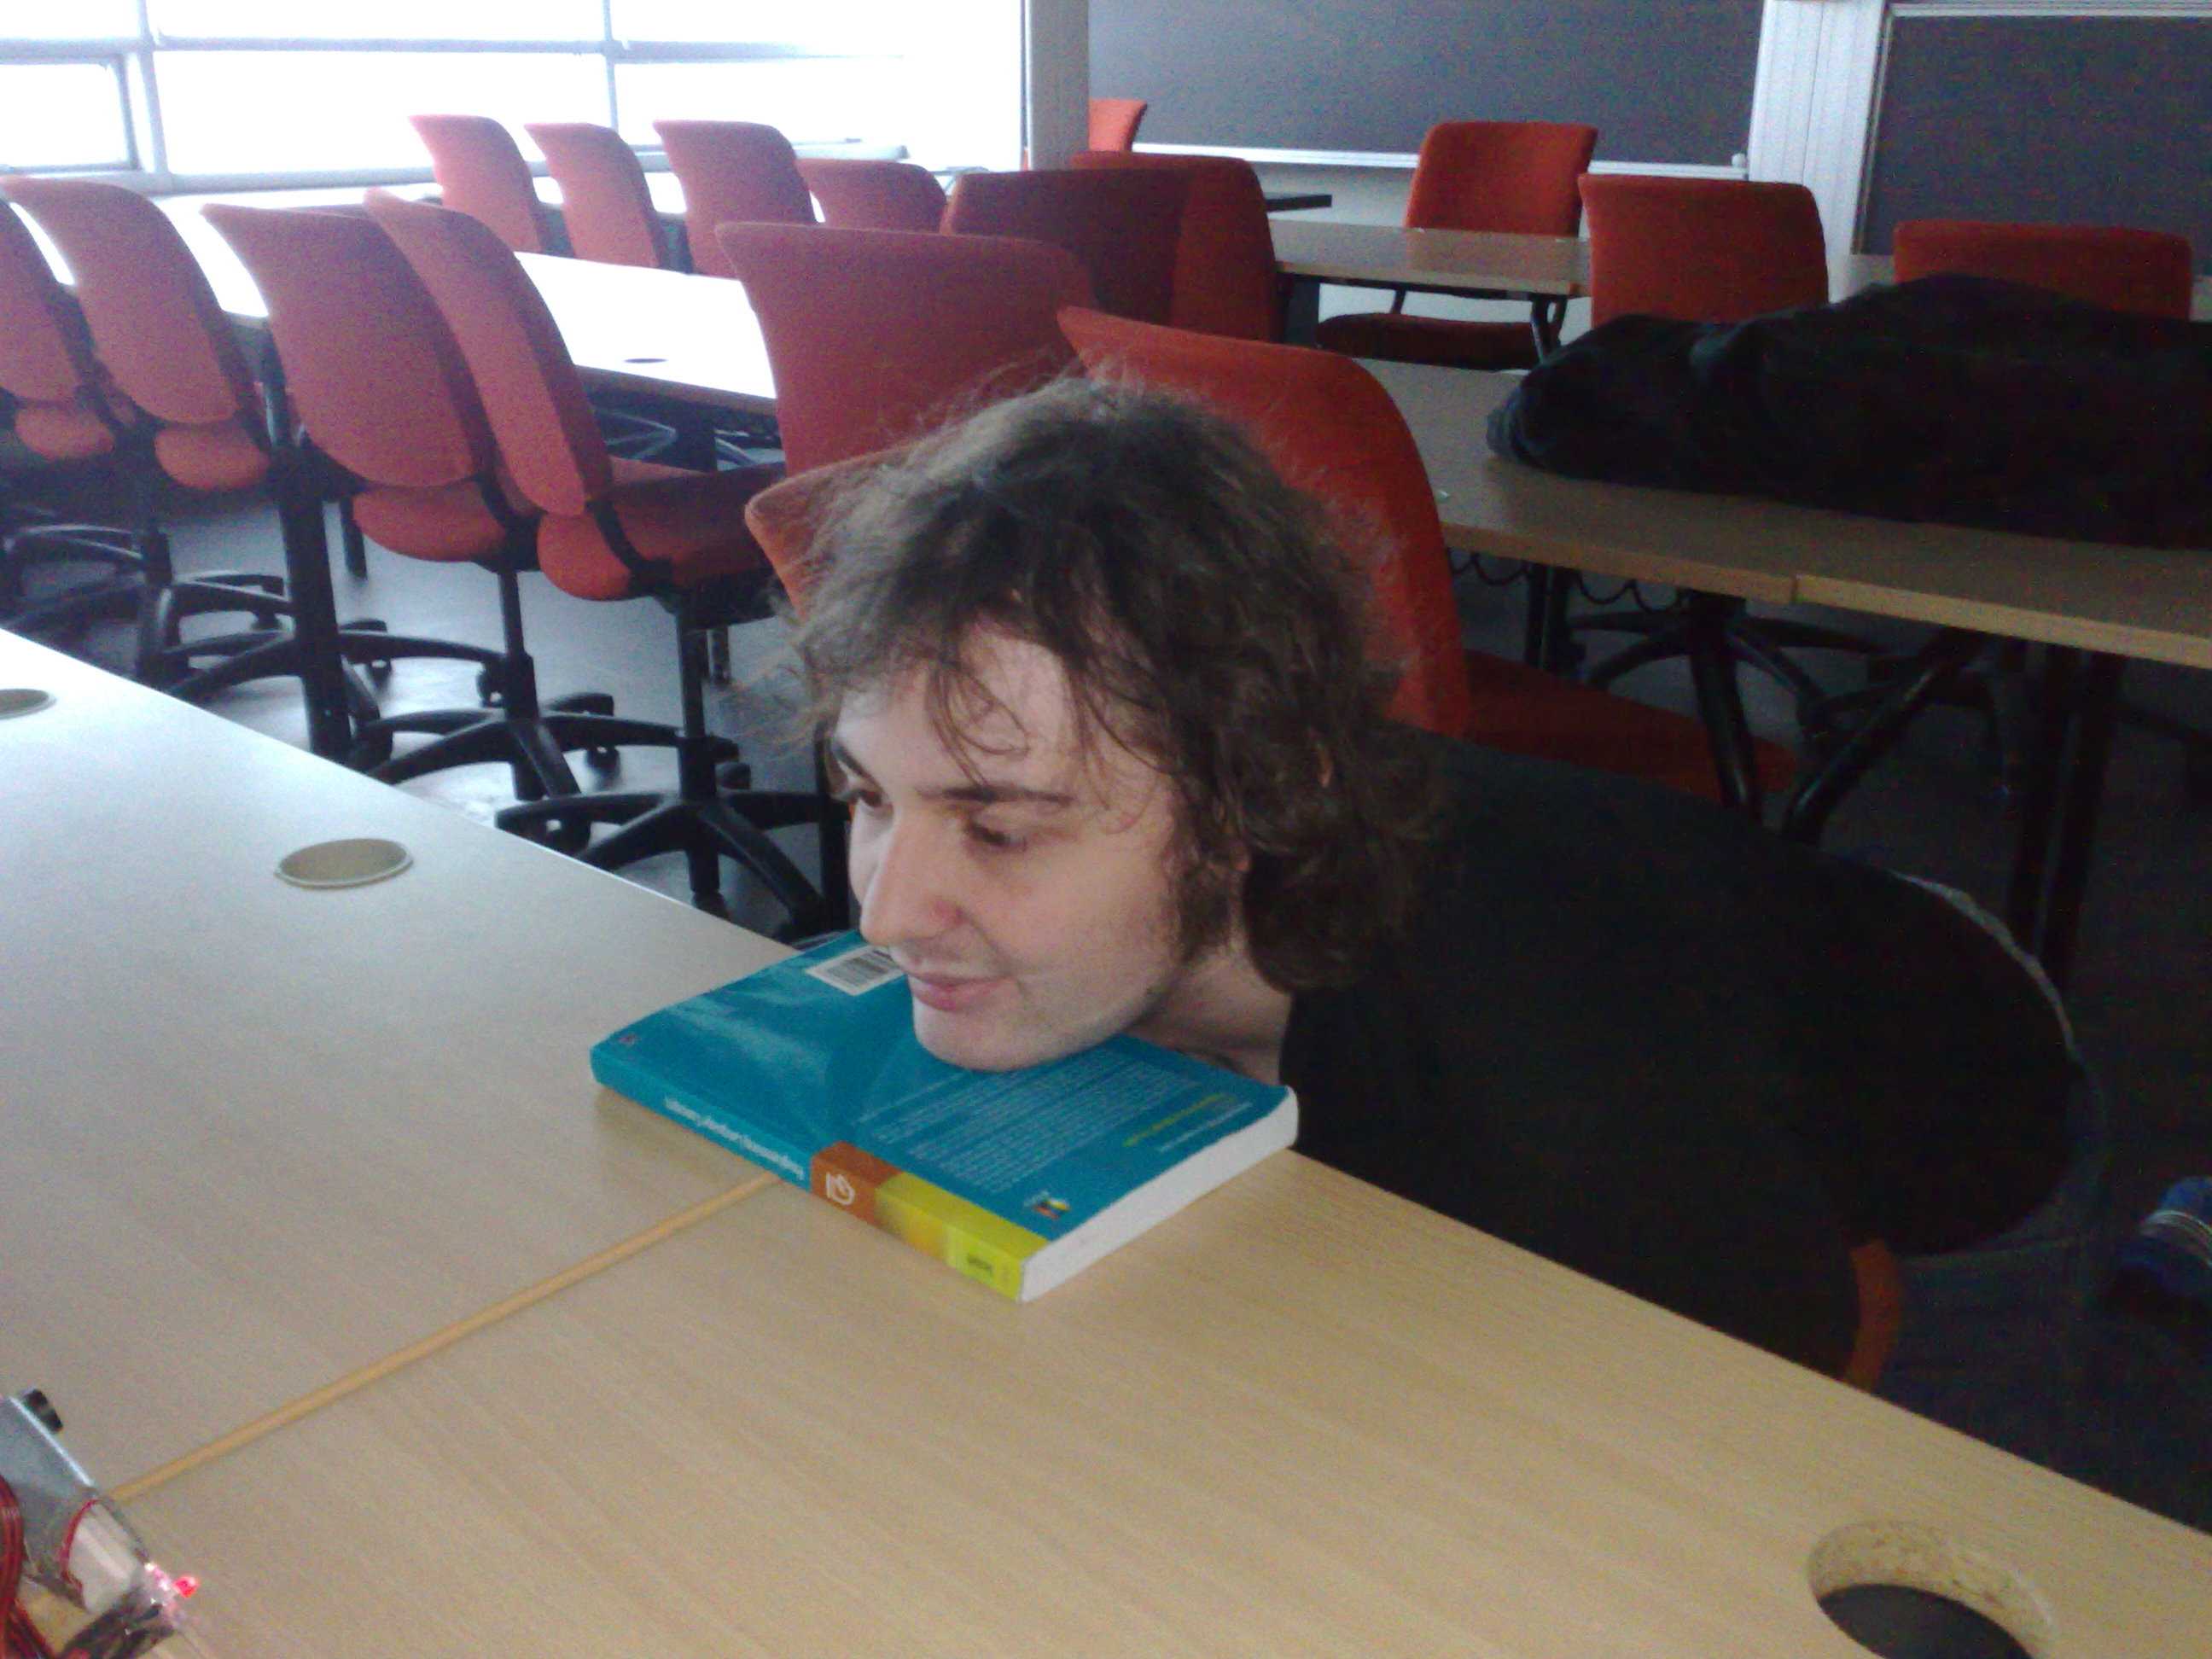
\includegraphics[width=0.6\textwidth]{mikkertest2}
\caption{Data gathering on test-subject.}
\label{fig:mikkertest2}
\end{figure}

\begin{figure}[h!]
\centering
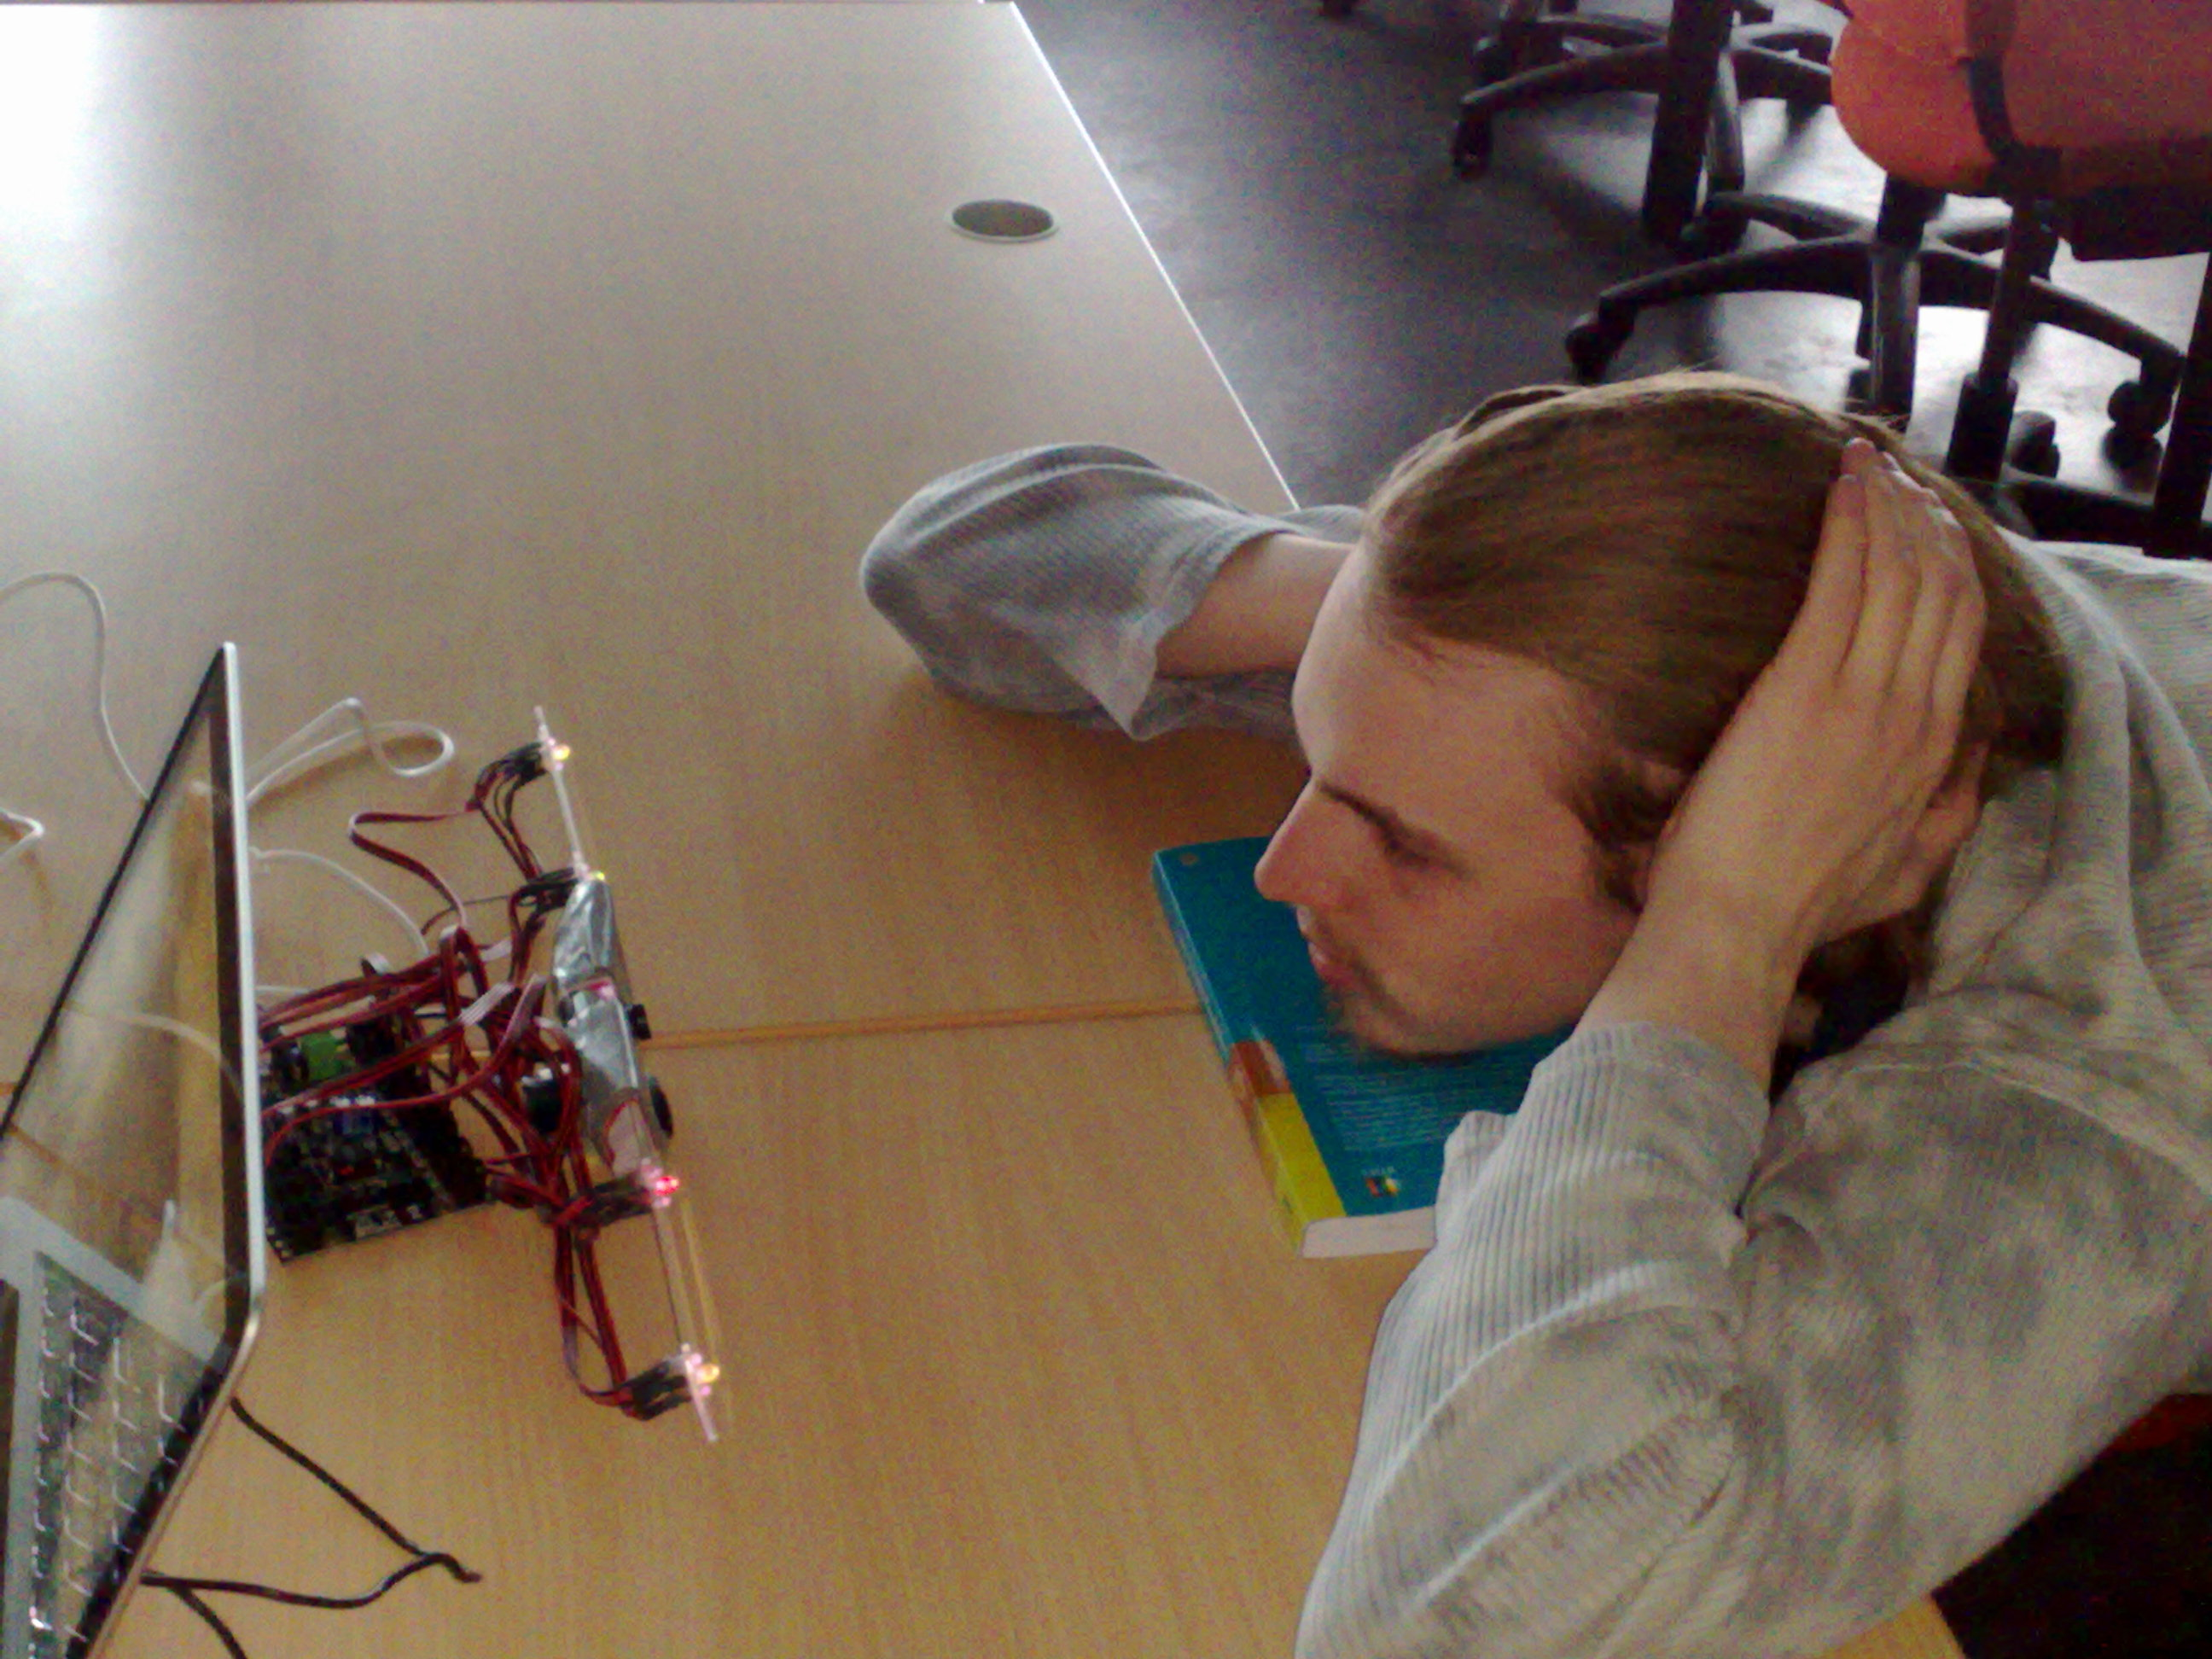
\includegraphics[width=0.6\textwidth]{spencertest}
\caption{Data gathering on test-subject.}
\label{fig:spencertest}
\end{figure}

\begin{figure}[h!]
\centering
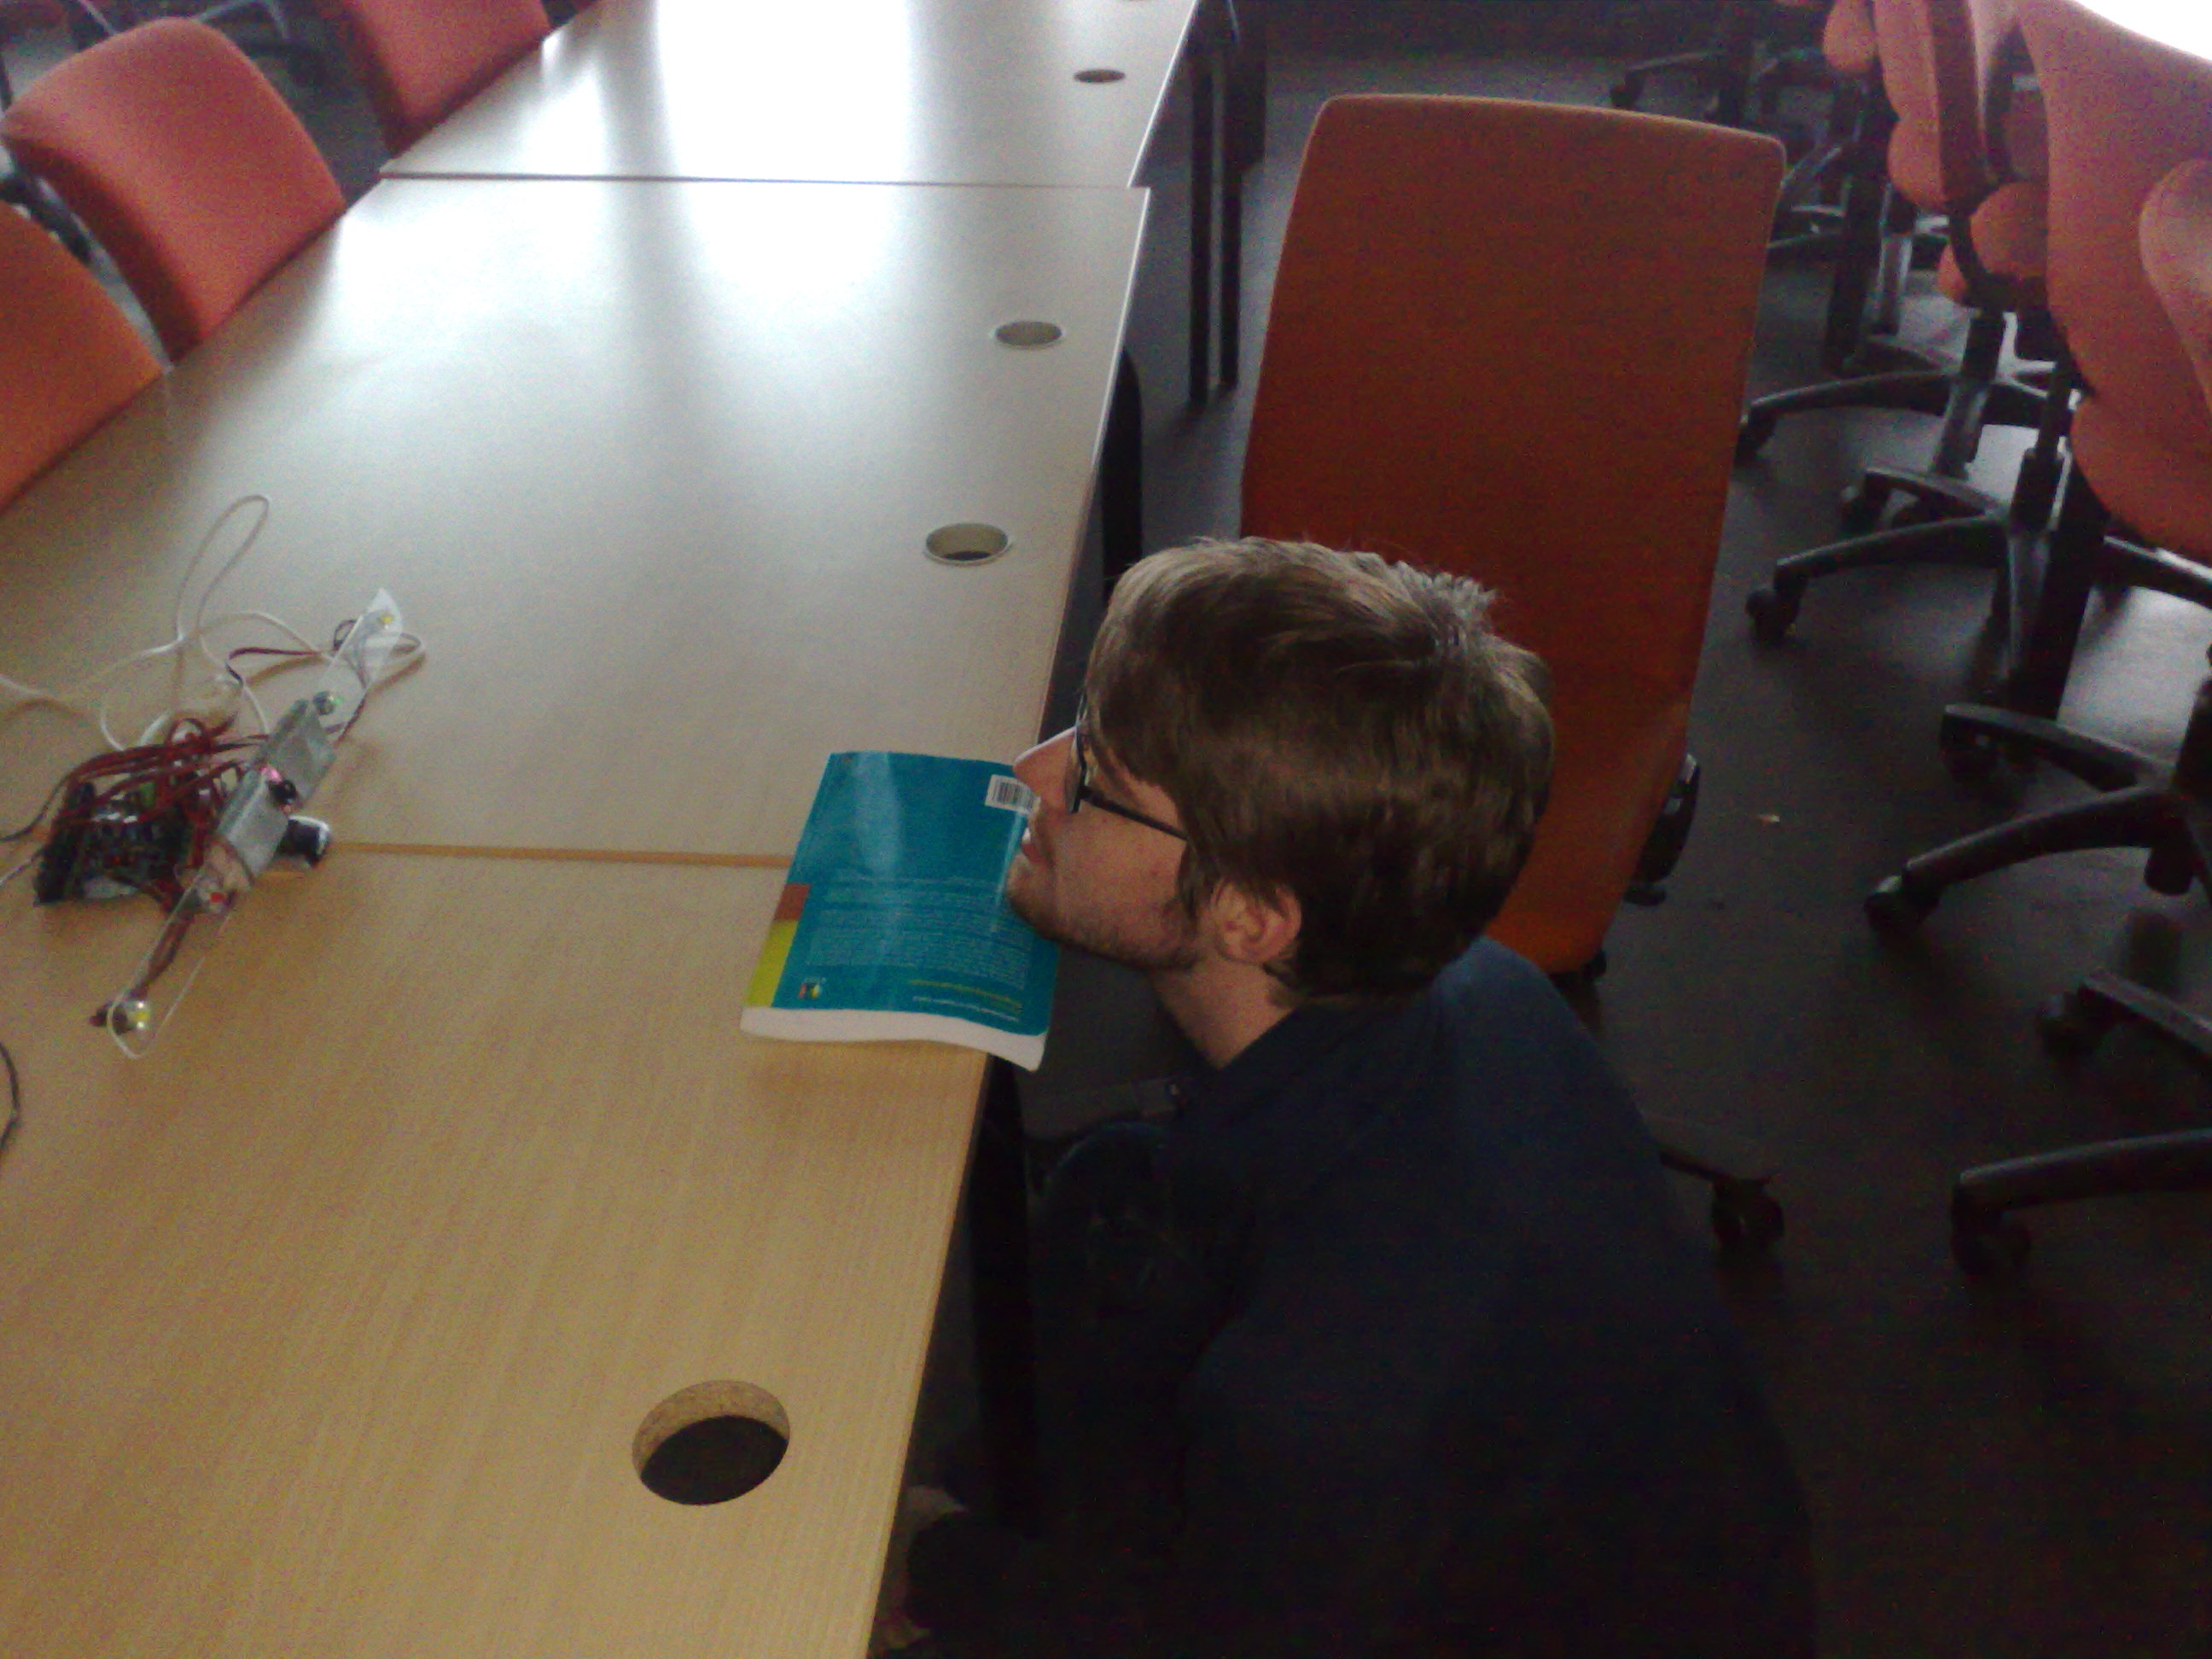
\includegraphics[width=0.6\textwidth]{petertest}
\caption{Data gathering on test-subject.}
\label{fig:petertest}
\end{figure}

\begin{figure}[h!]
\centering
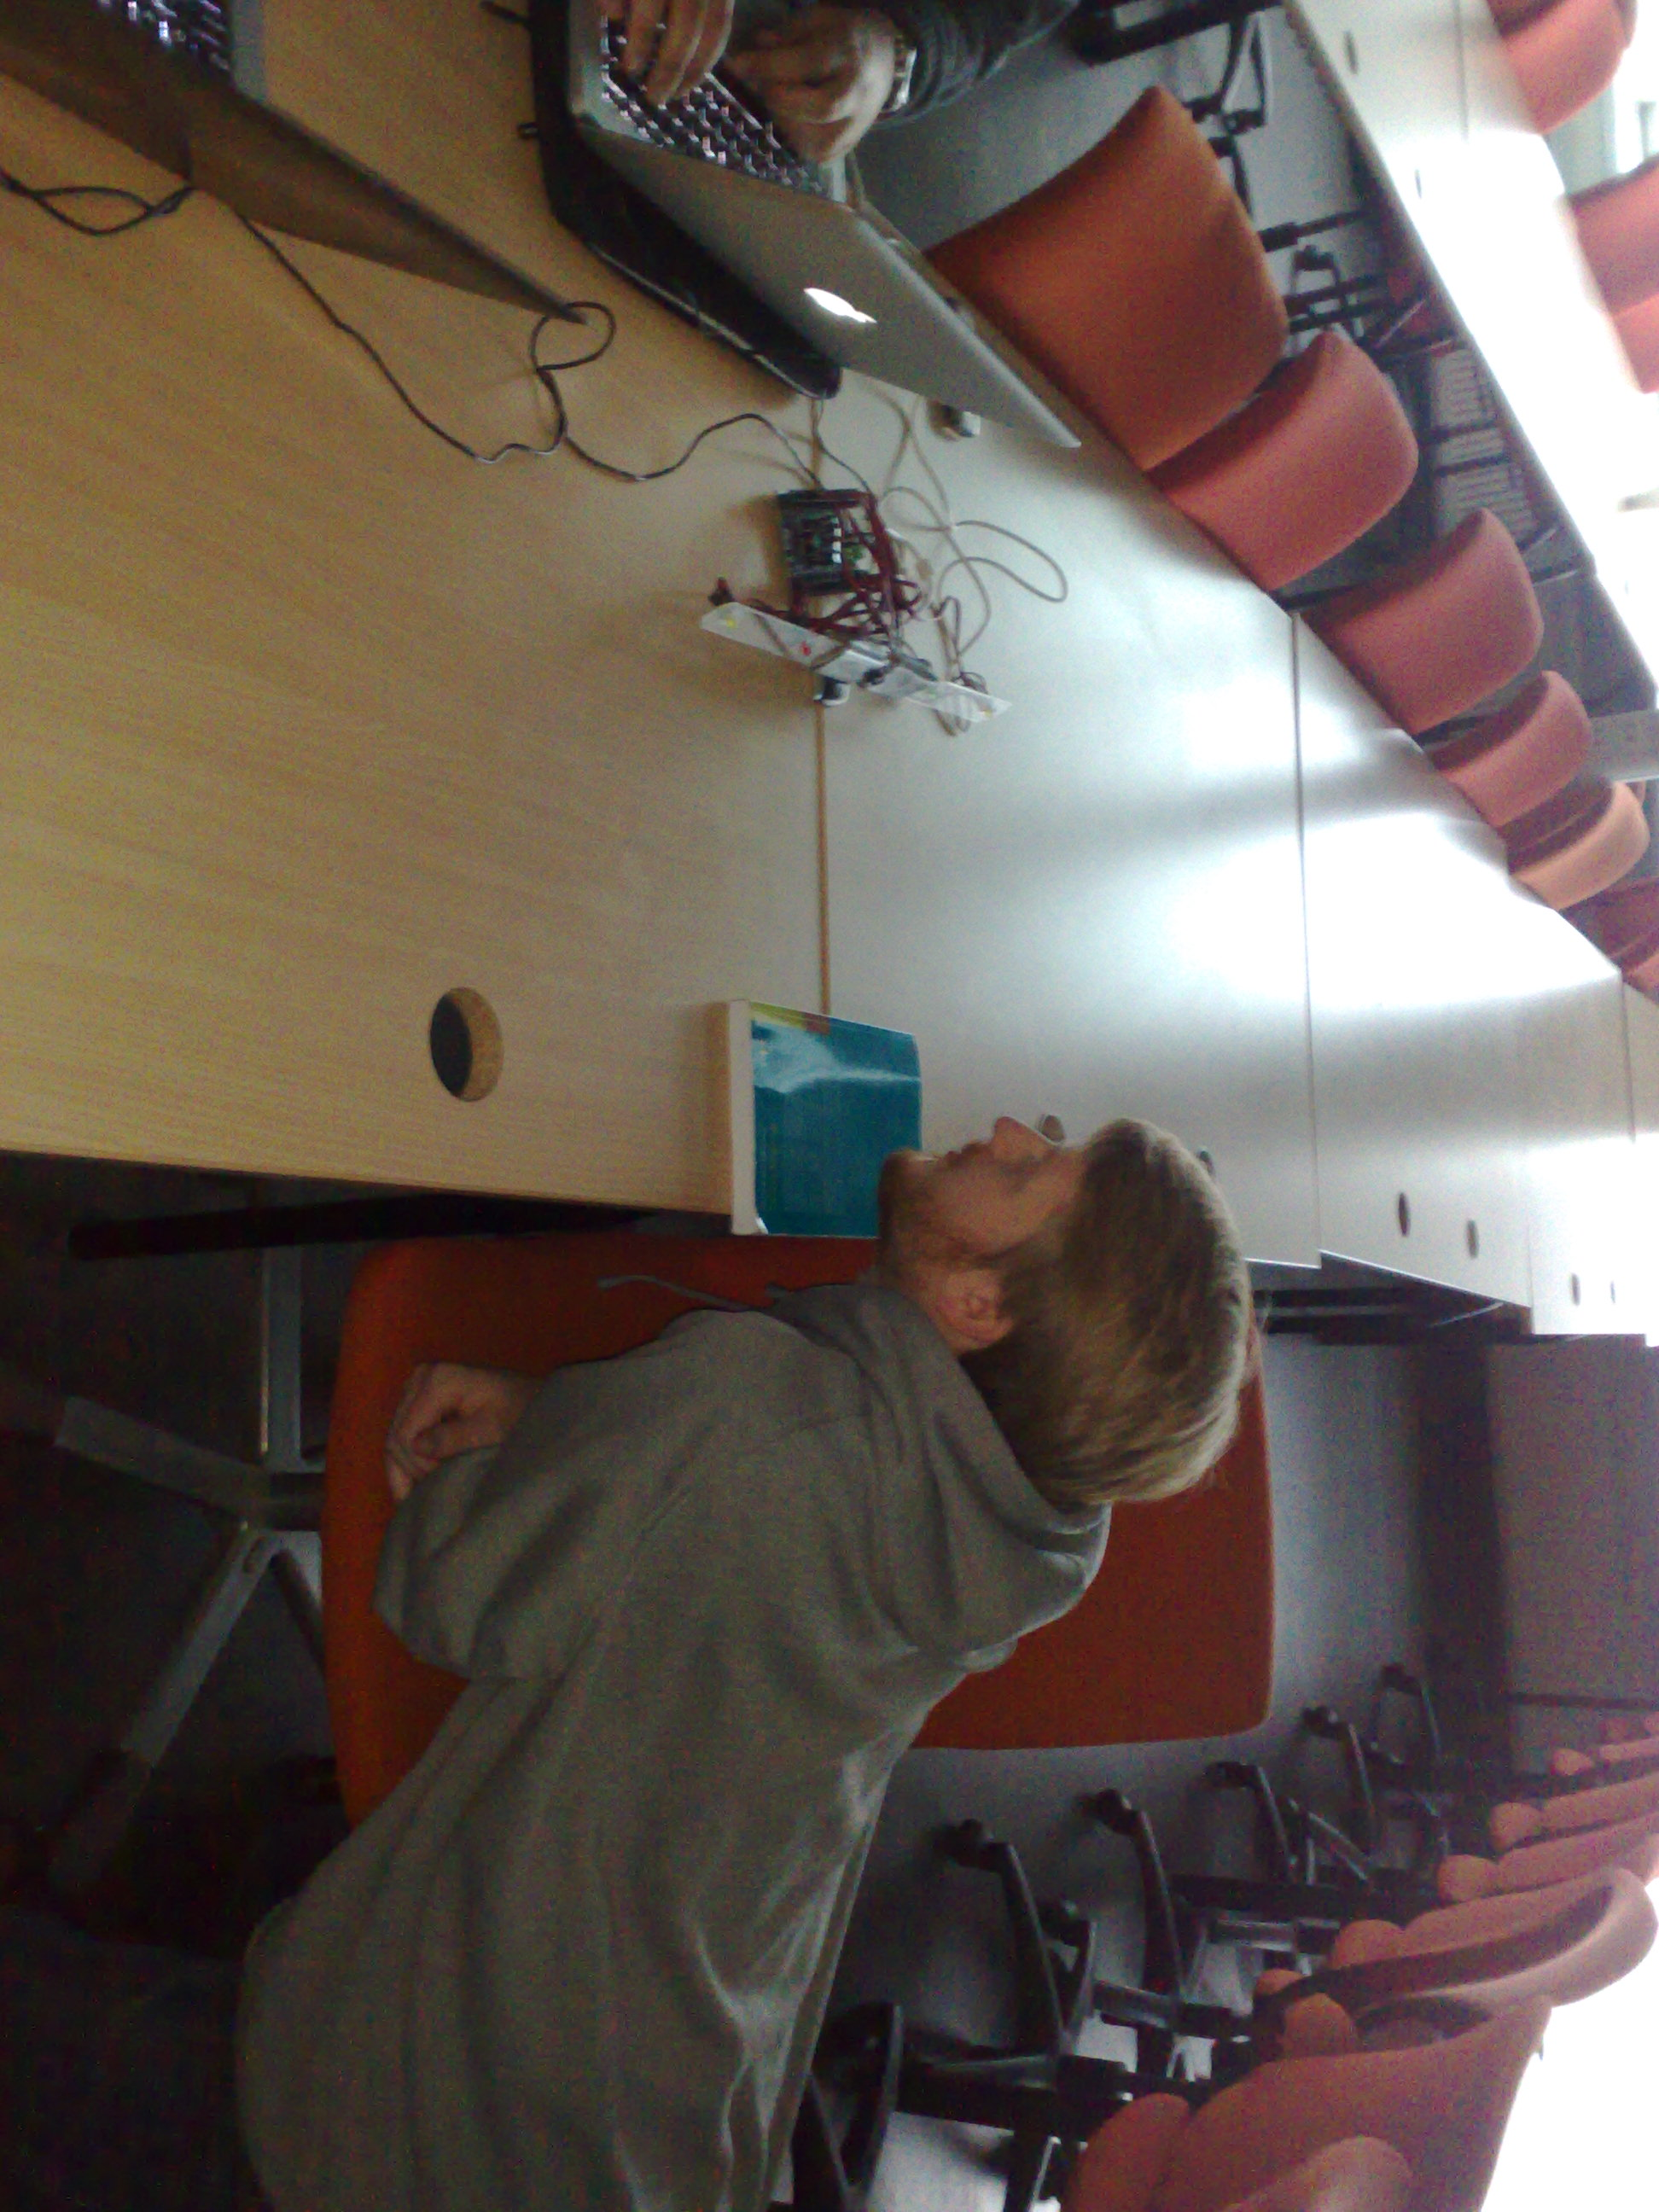
\includegraphics[angle=90,width=0.6\textwidth]{nielstest}
\caption{Data gathering on test-subject.}
\label{fig:nielstest}
\end{figure}
